\documentclass[12pt]{article}
\usepackage{latexsym}
\usepackage{epsfig}
\usepackage{amsmath}
\usepackage{amssymb}


\setlength{\topmargin}{0in}
\setlength{\leftmargin}{0in}
\setlength{\textwidth}{6in}
\setlength{\textheight}{9.5in}
\setlength{\parindent}{0.2in}
\setlength{\parskip}{.08in}
\voffset = -.45in
\hoffset = -.5in
\def\filledbox{\vrule height 1.8ex width .8ex depth -.1ex } % square bullet
\newcommand{\qed}{\large ~$\Box$ \normalsize}
%
%\newtheorem{thm}{Theorem}
%\newenvironment{theorem}{\begin{thm}\ \rm}{\end{thm}}
%
%\newtheorem{lem}{Lemma}
%\newenvironment{lemma}{\begin{lem}\ \rm}{\end{lem}}
%
\newtheorem{theorem}{Theorem}
\newtheorem{lemma}{Lemma}
\newtheorem{corollary}{Corollary}
\newenvironment{proof}{{\noindent \bf Proof\ \ }}{\qed}
\newenvironment{proofsketch}{{\noindent {\bf Proof}\ (sketch)\ \ }}{\qed}
%
\def\shh{\skew3\hat{\hat s}}
\def\dhh{\skew6\hat{\hat d}}
\begin{document}
\newcommand{\I}{\mbox{{\em Int}}}
\newcommand{\lt}{\mbox{{\em left}}}
\newcommand{\rt}{\mbox{{\em right}}}
\newcommand{\ld}{\Delta^l}
\newcommand{\rd}{\Delta^r}
\newcommand{\lsp}[1]{\large\renewcommand{\baselinestretch}{#1}\normalsize}
\newcommand{\hsp}{\hspace{.2in}}

\def\Endwhile{\mbox{\bf endwhile\ }}
\def\Or{\mbox{\bf or\ }}
\def\Do{\mbox{\bf do\ }}
\def\Downto{\mbox{\bf downto\ }}
\def\Int{\mbox{\bf int\ }}
\def\To{\mbox{\bf to\ }}
\def\Repeat{\mbox{\bf repeat\ }}
\def\Until{\mbox{\bf until\ }}
\def\Return{\mbox{\bf return\ }}
\def\Not{\mbox{\bf not\ }}
\def\And{\mbox{\bf and\ }}
\def\For{\mbox{\bf for\ }}
\def\Foreach{\mbox{\bf foreach\ }}
\def\Else{\mbox{\bf else\ }}
\def\Elseif{\mbox{\bf elseif\ }}
\def\End{\mbox{\bf end\ }}
\def\If{\mbox{\bf if\ }}
\def\Mod{\mbox{\bf \ mod\ }}
\def\Then{\mbox{\bf then\ }}
\def\While{\mbox{\bf while\ }}
\def\Output{\mbox{\bf output\ }}


\lsp{1}
\pagestyle{plain}
\begin{center}
{\bf
Prim Worksheet
}
\end{center}

\begin{figure}[h]
\center
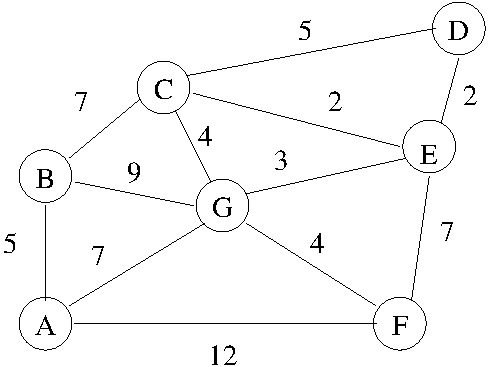
\includegraphics[width = 3in]{spanning.pdf}
\end{figure}

Start with vertex $A$ in a set by itself $T = \{A\}$ and with $T_{prim}$ 
empty. At each step, choose a vertex not in $T$ that can be joined to a 
vertex in $T$ using an edge of least cost. Add the vertex to $T$ and the
edge to $T_{prim}$. Show $T$ and $T_{prim}$ at the end of each iteration 

\begin{description}
\item [I1] 
\vspace*{0.25in}

\item [I2] 
\vspace*{0.25in}

\item [I3] 
\vspace*{0.25in}

\item [I4] 
\vspace*{0.25in}

\item [I5] 
\vspace*{0.25in}

\item [I6] 
\vspace*{0.25in}
\end{description}

\end{document}
